\documentclass[fleqn, a4paper, 12pt, twoside]{article}
\usepackage{exsheets} %question and solution environments
\usepackage{amsmath, amssymb, amsthm} %standard AMS packages
\usepackage{esint} %integral signs
\usepackage{marginnote} %marginnotes
\usepackage{gensymb} %miscellaneous symbols
\usepackage{commath} %differential symbols
\usepackage{xcolor} %colours
\usepackage{cancel} %cancelling terms
\usepackage{siunitx} %formatting units
\usepackage{tikz, pgfplots} %diagrams
	\usetikzlibrary{calc, hobby, patterns, intersections, angles, quotes, spy}
\usepackage{graphicx} %inserting graphics
\usepackage{epstopdf} %converting and inserting eps graphics
\usepackage{hyperref} %hyperlinks
\usepackage{datetime} %date and time
\usepackage{ulem} %underline for \emph{}
\usepackage{xfrac, lmodern} %inline fractions
\usepackage{enumerate, enumitem} %numbered lists
\usepackage{float} %inserting floats
\usepackage[american voltages]{circuitikz} %circuit diagrams
\usepackage{pdflscape}
\usepackage{setspace}
\usepackage{microtype}

\newcommand\numberthis{\addtocounter{equation}{1}\tag{\theequation}} %adds numbers to specific equations in non-numbered list of equations

\newcommand{\AxisRotator}[1][rotate=0]{
	\tikz [x=0.25cm,y=0.60cm,line width=.2ex,-stealth,#1] \draw (0,0) arc (-150:150:1 and 1);%
} %rotation symbols on axes

\theoremstyle{definition}
\newtheorem{example}{Example}
\newtheorem{definition}{Definition}

\theoremstyle{theorem}
\newtheorem{theorem}{Theorem}
\newtheorem{law}{Law}

\newcommand{\curl}{\mathrm{curl\,}}

\newcommand{\divergence}{\mathrm{div\,}}

\makeatletter
\@addtoreset{section}{part} %resets section numbers in new part
\makeatother

\newcommand\blfootnote[1]{%
	\begingroup
	\renewcommand\thefootnote{}\footnote{#1}%
	\addtocounter{footnote}{-1}%
	\endgroup
}

\SetupExSheets{solution/print = true} %prints all solutions by default

%opening
\title{Physics 2}
\author{Aakash Jog}
\date{\formatdate{24}{6}{2015}}

\begin{document}

\maketitle
%\setlength{\mathindent}{0pt}

\blfootnote
{	
	\begin{figure}[H]
		\includegraphics[height = 12pt]{cc.eps}
		\includegraphics[height = 12pt]{by.eps}
		\includegraphics[height = 12pt]{nc.eps}
		\includegraphics[height = 12pt]{sa.eps}
	\end{figure}
	This work is licensed under the Creative Commons Attribution-NonCommercial-ShareAlike 4.0 International License. To view a copy of this license, visit \url{http://creativecommons.org/licenses/by-nc-sa/4.0/}.
} %CC-BY-NC-SA license

\begin{question}
	\begin{figure}[H]
		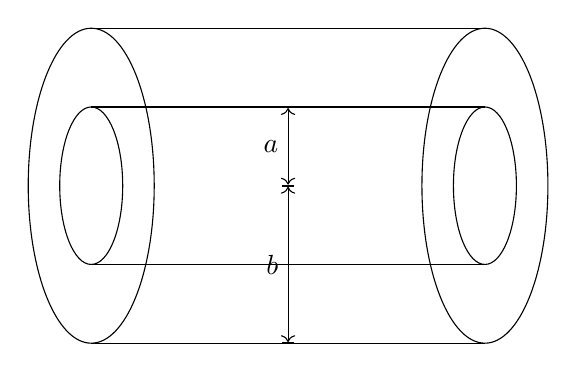
\begin{tikzpicture}
			\def\a{1};
			\def\b{2};
			\def\l{5};

			\draw (0,0) circle [x radius = 0.4*\a, y radius = \a];
			\draw (0,0) circle [x radius = 0.4*\b, y radius = \b];

			\draw (\l,0) circle [x radius = 0.4*\a, y radius = \a];
			\draw (\l,0) circle [x radius = 0.4*\b, y radius = \b];

			\draw (0,\a) -- (\l,\a);
			\draw (0,-\a) -- (\l,-\a);
			\draw (0,\b) -- (\l,\b);
			\draw (0,-\b) -- (\l,-\b);

			\begin{scope}[|<->|]
				\draw (\l/2,0) -- (\l/2,\a) node [midway, left] {$a$};
				\draw (\l/2,0) -- (\l/2,-\b) node [midway, left] {$b$};
			\end{scope}
		\end{tikzpicture}
	\end{figure}
	A cylindrical annular resistor with inner radius $a$ and outer radius $b$ has constant resistivity $\rho$.
	The two flat ends of the resistor are connected to a voltage source.
	What will be the net resistance?
\end{question}

\begin{solution}
	By the microscopic version of Ohm's Law,
	\begin{align*}
		\overrightarrow{j} & = \frac{1}{\rho} \overrightarrow{E}
	\end{align*}
	where $\rho$ is the resistivity.\\
	By the macroscopic version of Ohm's Law,
	\begin{align*}
		V            & = I R \\
		\therefore I & = \frac{V}{R}
	\end{align*}
	Therefore,
	\begin{align*}
		j                        & = \frac{1}{\rho} \frac{V}{l} \\
		\therefore \frac{I}{A}   & = \frac{V}{\rho l}           \\
		\therefore \frac{V}{R A} & = \frac{V}{\rho l}           \\
		\therefore R             & = \frac{\rho l}{A}
	\end{align*}
	As the flat ends of the resistor are connected to the voltage, the cylindrical annulus can be considered to be made up of cylindrical shells of varying radii, all connected in parallel.\\
	The resistance due to a cylindrical shell of radius $r$ is
	\begin{align*}
		\dif R & = \frac{\rho l}{2 \pi r \dif r}
	\end{align*}
	Therefore, as the shells are connected in parallel,
	\begin{align*}
		\frac{1}{R}  & = \int\limits_{a}^{b} \frac{1}{ \dif R}                   \\
                             & = \int\limits_{a}^{b} \frac{2 \pi r \dif r}{\rho l}       \\
                             & = \frac{2 \pi}{\rho l} \frac{\left( b^2 - a^2 \right)}{2} \\
		\therefore R & = \frac{\rho l}{\pi \left( b^2 - a^2 \right)}
	\end{align*}
\end{solution}

\begin{question}
	\begin{figure}[H]
		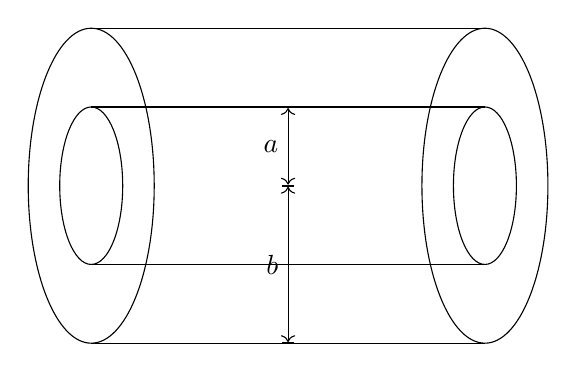
\begin{tikzpicture}
			\def\a{1};
			\def\b{2};
			\def\l{5};

			\draw (0,0) circle [x radius = 0.4*\a, y radius = \a];
			\draw (0,0) circle [x radius = 0.4*\b, y radius = \b];

			\draw (\l,0) circle [x radius = 0.4*\a, y radius = \a];
			\draw (\l,0) circle [x radius = 0.4*\b, y radius = \b];

			\draw (0,\a) -- (\l,\a);
			\draw (0,-\a) -- (\l,-\a);
			\draw (0,\b) -- (\l,\b);
			\draw (0,-\b) -- (\l,-\b);

			\begin{scope}[|<->|]
				\draw (\l/2,0) -- (\l/2,\a) node [midway, left] {$a$};
				\draw (\l/2,0) -- (\l/2,-\b) node [midway, left] {$b$};
			\end{scope}
		\end{tikzpicture}
	\end{figure}
	A cylindrical annular resistor with inner radius $a$ and outer radius $b$ has constant resistivity $\rho$.
	The inner and outer surfaces of the resistor are connected to a voltage source.
	What will be the net resistance?
\end{question}

\begin{solution}
	As the inner and outer surfaces of the resistor are connected to the voltage, the cylindrical annulus can be considered to be made up of cylindrical shells of varying radii, all connected in series.\\
	The resistance due to a cylindrical shell of radius $r$ is
	\begin{align*}
		\dif R & = \frac{\rho \dif r}{2 \pi r l}
	\end{align*}
	Therefore, as the shells are connected in series,
	\begin{align*}
		R & = \int\limits_{a}^{b} \dif R                        \\
                  & = \int\limits_{a}^{b} \frac{\rho \dif r}{2 \pi r l} \\
                  & = \frac{\rho}{2 \pi l} \ln \frac{b}{a}
	\end{align*}
\end{solution}

\begin{question}
	An infinite wire is carrying current $I_0$ to the right.
	A rectangular loop with resistance $k$ is kept in the plane of the wire is shown.
	\begin{figure}[H]
		\begin{tikzpicture}
			\def\l{2};
			\def\a{1};
			\def\R{1};

			\draw (-\l,0) -- (\l,0);

			\draw (-\l/2,\R) rectangle (\l/2,\R + \a);

			\begin{scope}[xshift = -20, |<->|]
				\draw (-\l/2,0) -- (-\l/2,\R) node [midway, left] {$R$};
				\draw (-\l/2,\R) -- (-\l/2,\R + \a) node [midway, left] {$a$};
			\end{scope}

			\begin{scope}[yshift = 20, |<->|]
				\draw (-\l/2,\R + \a) -- (\l/2,\R + \a) node [midway, above] {$l$};
			\end{scope}
		\end{tikzpicture}
	\end{figure}
	The loop is moving upwards with a constant velocity $v$.\\
	Find the current induced in the loop.
\end{question}

\begin{solution}
	As the current is flowing to the right, the magnetic field at any point above the wire is directed outwards.\\
	Consider an elemental rectangular area of length $l$ and height $\dif r$, at height $r$ from the wire.\\
	Therefore,
	\begin{align*}
		\dif \Phi_B & = B \dif A                                          \\
                            & = \left( \frac{\mu_0 I}{2 \pi r} \right) (l \dif r) \\
	\end{align*}
	Therefore,
	\begin{align*}
		\Phi_B & = \int\limits_{R}^{R + a} \frac{\mu_0 I}{2 \pi r} l \dif r         \\
                       & = \frac{\mu_0 I l}{2 \pi} \int\limits_{R}^{R + a} \frac{\dif r}{r} \\
                       & = \frac{\mu_0 I l}{2 \pi} \ln \frac{R + a}{R}                      \\
                       & = \frac{\mu_0 I l}{2 \pi} \left( \ln(R + a) - \ln(R) \right)
	\end{align*}
	As the loop is moving upwards, $B$ is changing.
	Therefore, $\Phi_B$ is also changing.\\
	Therefore,
	\begin{align*}
		\dod{\Phi_B}{t} & = \dod{}{t}\left( \frac{\mu_0 I l}{2 \pi} \left( \ln(R + a) - \ln(R) \right) \right)     \\
                                & = \frac{\mu_0 I l}{2 \pi} \dod{}{t} \left( \ln(R + a) - \ln(R) \right)                   \\
                                & = \frac{\mu_0 I l}{2 \pi} \left( \frac{1}{R + a} \dod{}{t}(R + a) - \dod{}{t}(R) \right) \\
                                & = \frac{\mu_0 I l}{2 \pi} \left( \frac{1}{R + a} v - \frac{1}{R} v \right)               \\
                                & = \frac{\mu_0 I l v}{2 \pi} \left( \frac{1}{R + a} - \frac{1}{R} \right)
	\end{align*}
	Therefore, by Faraday's Law,
	\begin{align*}
		|\varepsilon| & = \left| \dod{\Phi_B}{t} \right| \\
                              & = \frac{\mu_0 I l v}{2 \pi} \left( \frac{1}{R} - \frac{1}{R + a} \right)
	\end{align*}
	Therefore,
	\begin{align*}
		I & = \frac{\varepsilon}{k} \\
                  & = \frac{\mu_0 I l v}{2 \pi k} \left( \frac{1}{R} - \frac{1}{R + a} \right)
	\end{align*}
	As the loop moves upwards, the magnetic flux through it is increasing.\\
	Therefore, by Lenz's Law, the induced current will be such that the magnetic field due to this current acts to increase the magnetic flux.\\
	Therefore, the induced current is anti-clockwise.
\end{solution}

\begin{question}
	An infinite plane with surface charge density $\sigma$ is kept on the $x$-$y$ plane.
	The plane is moving with a constant velocity $\overrightarrow{v} = v \hat{i}$.\\
	Find the magnetic field everywhere.
\end{question}

\begin{solution} 
	As the charge density is moving with $v$,
	\begin{align*}
		k & = \sigma v
	\end{align*}
	where $k$ is the current per unit length.\\
	Consider a square virtual Ampere loop, directed anti-clockwise, as shown.
	\begin{figure}[H]
		\begin{tikzpicture}
			\def\xMIN{-5};
			\def\xMAX{5};
			\def\yMIN{-2};
			\def\yMAX{2};

			\def\l{2};
			\def\h{3};

			\begin{scope}[stealth-stealth, lightgray]
				\draw (\xMIN,0) -- (\xMAX,0) node [right] {$y$};
				\draw (0,\yMIN) -- (0,\yMAX) node [above] {$z$};
			\end{scope}

			\begin{scope}
				\draw (-\l/2,-\h/2) rectangle (\l/2,\h/2);
			\end{scope}

			\begin{scope}
				\foreach \x in {\xMIN,...,\xMAX}
				{
					\node at (\x,0) {$\odot$};
				}
			\end{scope}
		\end{tikzpicture}
	\end{figure}
	Therefore by Ampere's Law,
	\begin{align*}
		\oint \overrightarrow{B} \cdot \overrightarrow{\dif l} & = \mu_0 I_{\textnormal{enclosed}} \\
		\therefore 2 |B| l                                     & = \mu_0 k l                       \\
		\therefore |B|                                         & = \frac{\mu_0 k}{2}
	\end{align*}
	Therefore,
	\begin{align*}
		\overrightarrow{B} &=
			\begin{cases}
				-\frac{\mu_0 k}{2} \hat{y} & ;\quad z > 0 \\
				\frac{\mu_0 k}{2} \hat{y}  & ;\quad z < 0 \\
			\end{cases}
	\end{align*}
	Therefore,
	\begin{align*}
		\overrightarrow{B} &=
			\begin{cases}
				-\frac{\mu_0 \sigma v}{2} \hat{y} & ;\quad z > 0 \\
				\frac{\mu_0 \sigma v}{2} \hat{y}  & ;\quad z < 0 \\
			\end{cases}
	\end{align*}
\end{solution}

\end{document}
